\documentclass[12pt]{article}
\usepackage{graphicx,fullpage}
\pagestyle{plain}
\headheight0in
\headsep0in
\topmargin -0.1in
\textheight 9.0in
\oddsidemargin -0.0in
\textwidth 6.5in
\baselineskip 3ex
\renewcommand\baselinestretch{1}
\parindent 0in
\parskip 0.1in
\def\bc{\begin{center}}
\def\ec{\end{center}}
\def\qskip{\vspace{1.5in}}
\begin{document}
\begin{center}
{\bf Statistics 531/Econ 677\\

Winter, 2007\\

Ed Ionides\\
\vspace{7 mm}
Name: \hrulefill UMID \#: \hrulefill\\
\vspace{7 mm}
Midterm Exam}
\end{center}
{\bf There are 3 sections (A, B and C) containing a total of 11 questions worth
26 points. Points will be awarded for clearly explained and accurate answers. You may use the course textbook, the course notes and a calculator.}\\
\begin{center}
\renewcommand{\arraystretch}{2}
\begin{tabular}{||c|c|c||}
\hline
\hline
{Section} & {Points} & {Score}\\
\hline
\hline
A & 6 & \\
\hline
B & 6 & \\
\hline
C & 14 & \\
\hline
\hline
Total & 26 &  \\
\hline
\hline
\end{tabular}
\end{center}
\newpage

We investigate over-crowding in the Emergency Room of the University of Michigan Hospital.
The data, $x_t$, are hourly occupancy fractions for one year, starting July 1st 2005. Occupancy fraction is defined to be the mean number of patients in the ER during each hour  divided by the total number of beds available (the ER operates 24 hours a day, 7 days a week, 365 days a year).
Note that the occupancy fraction, shown in Fig.~\ref{fig:er}, can exceed one.
The purposes of investigating these data are to predict future occupancy, and to make progress toward relating ER overcrowding with other variables such as errors in medical procedures.
\begin{figure}[h]
\bc
%\vspace{-0.5cm}
\vspace{-1cm}
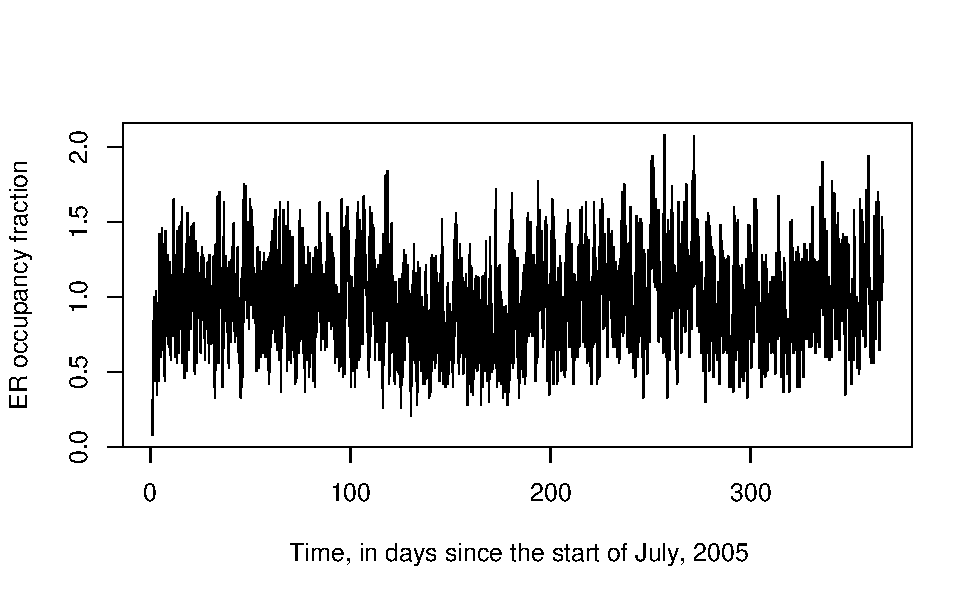
\includegraphics[width=5in]{ER-um-05}
%\vspace{-0.5cm}
\vspace{-1cm}
\ec
\caption{Hourly occupancy fraction at the University of Michigan Emergency Room}\label{fig:er}
\end{figure}

{\bf SECTION A}. Fig.~\ref{fig:summary} shows a smoothed periodogram and an ACF of the data.
\begin{figure}
\vspace{-1cm}
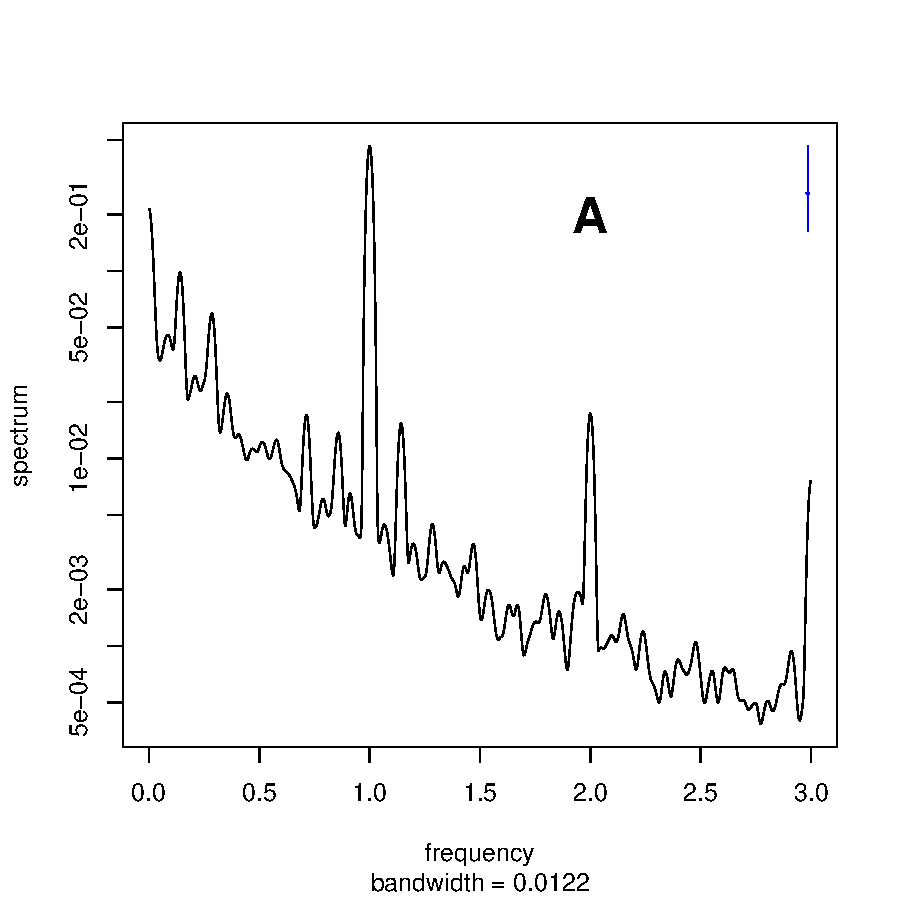
\includegraphics[width=3in,height=3in]{ER-um-spec-closeup}
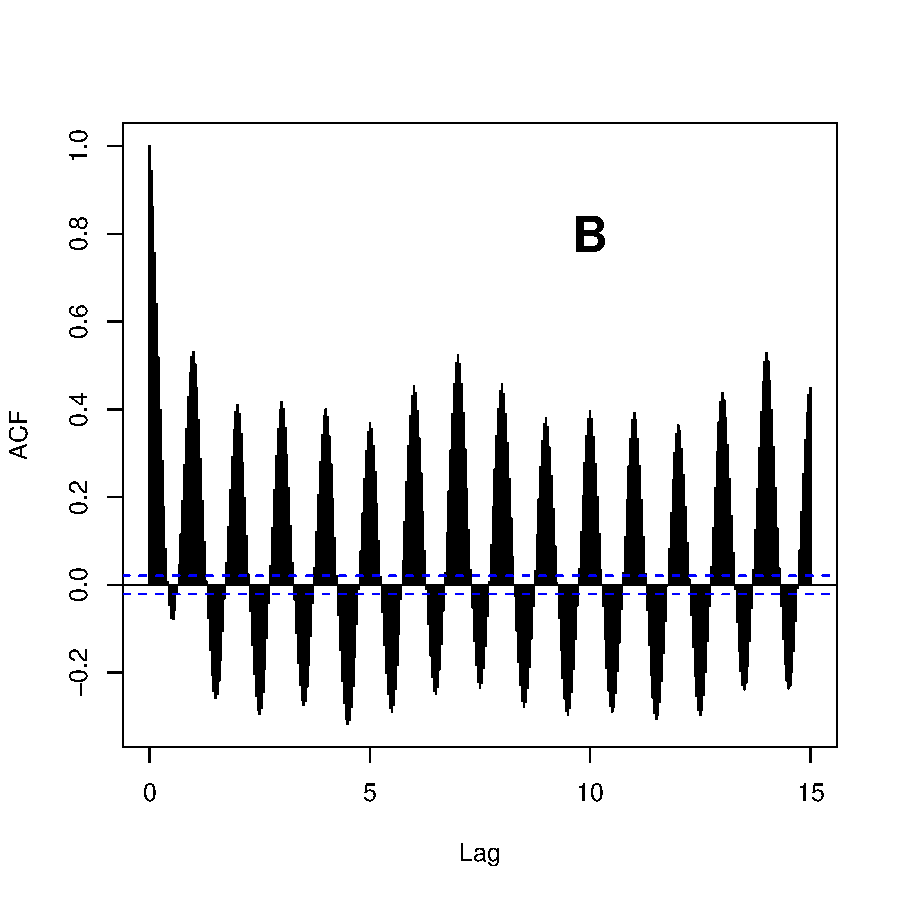
\includegraphics[width=3in,height=3in]{ER-um-acf}
\vspace{-0.5cm}
\caption{(A) Smoothed periodogram of $x_t$. (B) sample auto-covariance function of $x_t$}\label{fig:summary}
\end{figure}

A1. [1 point] What are the units of frequency in Fig.~\ref{fig:summary}A? 
Explain your reasoning.
\qskip

A2. [2 points] Explain how you can tell that the periodogram in Fig.~\ref{fig:summary}A has been truncated to exclude high frequencies (this is done to highlight the information about lower frequencies).

\qskip

\newpage

%A3. [2 points] Explain why Fig.~\ref{fig:summary} shows that the weekly pattern is (at most) a minor effect.
%\qskip

A3. [3 points] Using Fig.~\ref{fig:summary}, can you reject a null hypothesis that there is no weekly pattern to occupancy fraction? Explain.

% to carry out an approximate hypothesis test
%, at a significance level of 0.05,  
%of the null hypothesis that there is no weekly effect.

\qskip

\vspace{2cm}

{\bf SECTION B}. 
Fig.~\ref{fig:er} suggests that the occupancy could be modeled by a random process whose expected value $\mu_t$ is slowly varying with time.
%B1. [2 points] Could this variation be an annual cycle? Explain.
%\qskip
The variation around the mean in  Fig.~\ref{fig:er} appears quite stable.
 Thus, it may be reasonable to suppose that $x_t-\mu_t$ is stationary, where $\mu_t=E[x_t]$.
We can estimate $\mu_t$ %by an estimate $\hat \mu_t$ found 
using local regression. This is done here using the R command \texttt{mu.hat=loess(x}$ \sim$ \texttt{time,span=0.5)\$fitted}. The estimate $\hat \mu_t$ of $\mu_t$ is shown in Fig.~\ref{fig:smo}.
\begin{figure}[h]
\bc
\vspace{-1cm}
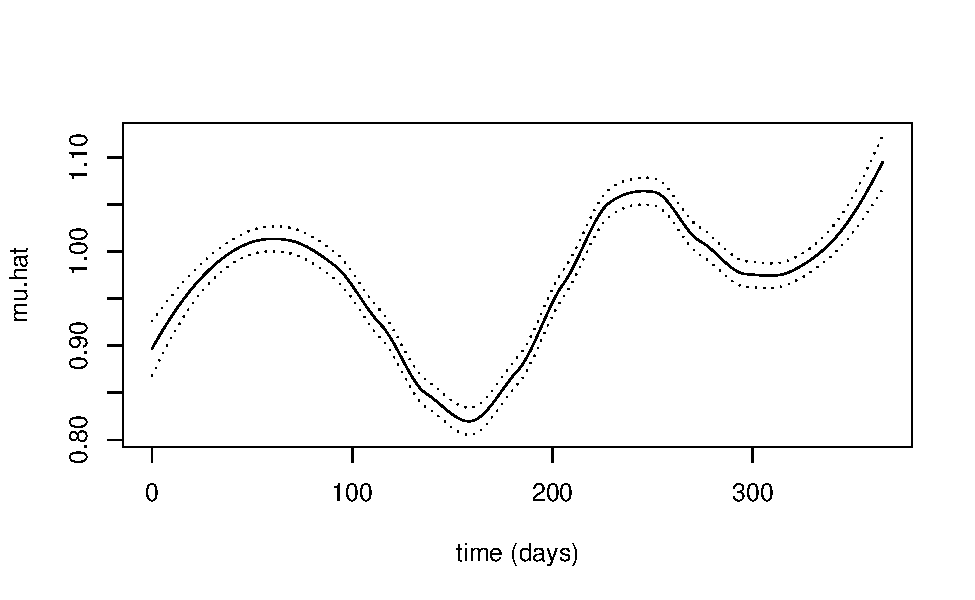
\includegraphics[width=4.5in]{ER-um-smo}
\vspace{-1cm}
\ec
\caption{Estimate $\hat\mu_t$ of the mean hourly occupancy fraction $\mu_t$.}\label{fig:smo}
\end{figure}

B1. [2 points] Briefly describe what ``local regression estimate'' means.

\qskip

\newpage

B2. [2 points] The dashed lines in Fig.~\ref{fig:smo} show an approximate 95\% confidence interval, constructed by adding $\pm 2SE$ where $SE$ is the standard error on the estimate of the mean, as calculated by the local regression. Is this interval appropriate? Explain. You should be able to comment even without a detailed understanding of local regression.

\qskip

B3. [2 points] Could the data be consistent with a model where the mean is not varying with time, e.g. a stationary process? Say yes or no, and explain.

\qskip

%B4. Does the removed trend function contain weekly or daily effects at noticeable levels? One way to look at this is to calculate the periodogram of $\hat\mu_t$.

{\bf SECTION C}. We investigate the stationarity of the detrended occupancy fraction $y_t=x_t-\hat\mu_t$. In particular, we compare the two time intervals  August/September 2005 and March/April 2006.
First, we fit an $ARIMA(1,0,1){\times}(1,0,1)_{24}$ model to the 61 days in August and September 2005. Below is the R output.

\newpage
\begin{verbatim}
arima(x = y[AugSep], order = c(1, 0, 1), seasonal = c(1, 0, 1))
Coefficients:
         ar1     ma1    sar1     sma1  intercept
      0.9139  0.0403  0.9998  -0.9884    -0.0060
s.e.  0.0114  0.0277  0.0002   0.0080     0.1354
sigma^2 estimated as 0.006561:  log likelihood = 1568.48,  aic = -3124.96
\end{verbatim}
C1. [3 points] Write out the fitted model, carefully stating all the model assumptions.

\qskip

\begin{figure}[ht]
%\vspace{-1cm}
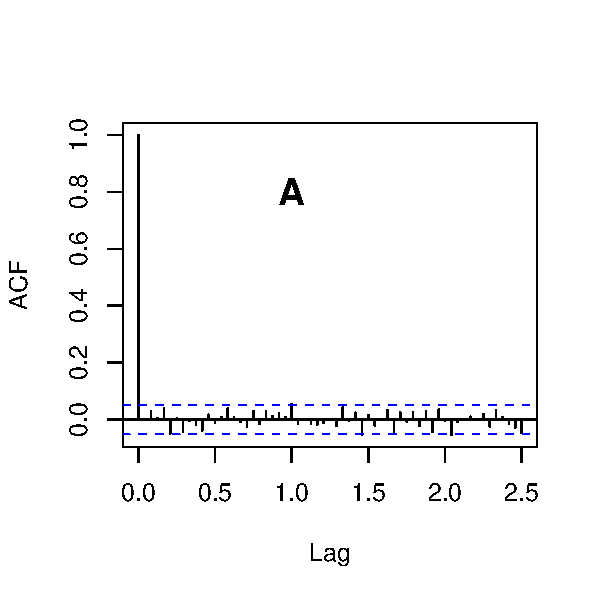
\includegraphics[width=3in,height=2.5in]{ER-resid-acf}
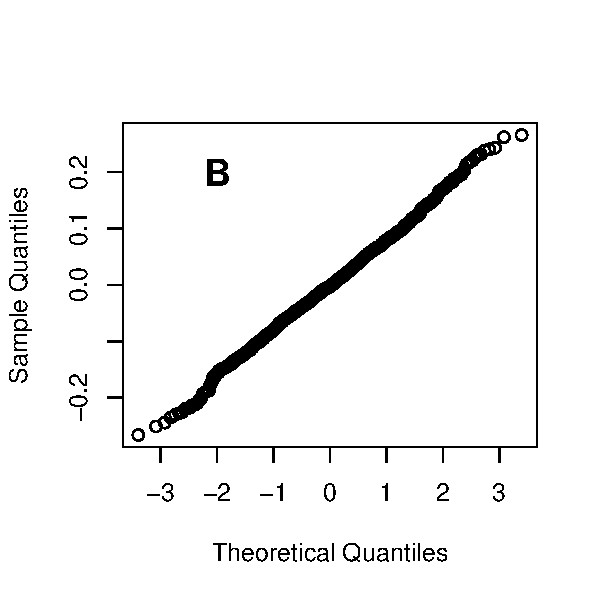
\includegraphics[width=3in,height=2.5in]{ER-qqnorm}
\vspace{-0.5cm}
\caption{ Investigation of the residuals from fitting an $ARIMA(1,0,1){\times}(1,0,1)_{24}$ model to August/September. (A) Sample ACF. (B) normal quantile plot.}\label{fig:diag}
\end{figure}
C2. [3 points] What do you conclude from the diagnostic plots in Fig.~\ref{fig:diag}? Also, explain at least one relevant property that is NOT checked by these diagnostic plots, and describe how you could check it.

\qskip

\newpage

C3. [2 points] Based on  Fig.~\ref{fig:diag} and the R model output above,  $ARIMA(1,0,1){\times}(0,1,1)_{24}$ was considered to be an acceptable model. Explain the reasoning.

\qskip
\vspace{1cm}

C4. [2 points] A comparison of various models is presented in Table~\ref{tab:aic}. What do you conclude from the AIC values in Table~\ref{tab:aic}, together with the previous value of -3124.96 for $ARIMA(1,0,1){\times}(1,0,1)_{24}$?


\qskip
\qskip
%\vspace{1cm}

\begin{table}[ht]
A.\begin{tabular}{c|rrr}
$p\setminus q$ &     0 &    1 &    2 \\
\hline
 0&     NA &-1612.9 &-2258.7\\
 1&-3060.0 &-3058.8 &-3057.2\\
 2&-3058.8 &-3057.1 &-3055.2\\
3&-3057.2 &-3054.8 &-3059.1
\end{tabular}
\hspace{0.5in} 
B. \begin{tabular}{c|rrr}
 $p\setminus q$ &     0 &    1 &    2 \\
\hline
 0&     NA &-1168.5 &-1844.2\\
 1&-2944.9 &-2944.4 &-2943.2\\
 2&-2944.5 &-2943.1 &-2941.3\\
3 &-2943.2 &-2941.3 &-2939.8
\end{tabular}
\caption{AIC values from fitting $ARIMA(p,0,q){\times}(0,1,1)_{24}$ models to (A) August/September 2005, (B) March/April 2006.}\label{tab:aic}
\end{table}   

\newpage
Below is the R output from fitting an $ARIMA(1,0,0){\times}(0,1,1)_{24}$ model to August/September 2005 and March/April 2006.
\begin{verbatim}
arima(x = y[AugSep], order = c(1, 0, 0), seasonal = c(0, 1, 1))
Coefficients:
         ar1     sma1
      0.9195  -1.0000
s.e.  0.0104   0.0197
sigma^2 estimated as 0.006496:  log likelihood = 1533,  aic = -3060
\end{verbatim}
\begin{verbatim}
arima(x = y[MarApr], order = c(1, 0, 0), seasonal = c(0, 1, 1))
Coefficients:
         ar1     sma1
      0.9436  -1.0000
s.e.  0.0088   0.0341
sigma^2 estimated as 0.007036:  log likelihood = 1475.46,  aic = -2944.92
\end{verbatim}


C5. [4 points] Show how to carry out an approximate hypothesis test that the AR1 component is the same for August/September 2005 and March/April 2006 in the context of an
 $ARIMA(1,0,0){\times}(0,1,1)_{24}$ model. 
Explain what your approximations are for this test. How good do you think these approximations are, and how could you check?
Note: since you are not provided with statistical tables, you are not required to calculate a p-value.


\qskip

\qskip

\end{document}
